\documentclass[hidelinks]{article}
\usepackage{fontspec}
\usepackage{minted}
\usepackage{indentfirst}
\usepackage{xcolor}
\usepackage{soul}
\usepackage{graphicx}
\graphicspath{{../imgs}}
\usepackage{blindtext}
\usepackage{hyperref}
\usepackage{amsmath}
\usepackage{cleveref}
\usepackage{placeins}
\usepackage[letterpaper, portrait, margin=1in]{geometry}
\usemintedstyle{xcode}
\renewcommand\theFancyVerbLine{\small\arabic{FancyVerbLine}}
\newfontfamily\cascadiacodefont{Cascadia Code}[NFSSFamily=CascadiaCodeFamily]
\setminted{linenos, fontfamily=CascadiaCodeFamily, frame=lines, breaklines}

\title{ME 3313 Honors Project}

\definecolor{lightgreen}{HTML}{8EE0B6}

\definecolor{lightblue}{HTML}{34B1EB}

\begin{document}
    \begin{flushleft}
        Nat Curtis
        
        ME 3313
        
        9/10/2025
    \end{flushleft}

    \begin{center}
        \Large ME 3313 Honors Project
    \end{center}


    \FloatBarrier\section*{Introduction}

    For this project, I am analyzing the linkages of a skid-steer bucket loader, shown in \autoref{fig:sideview}. I will explore each of the topics we explore in ME 3313, starting with mobility, and going on to topics including range of motion, position, velocity, acceleration, and forces, and use each of these topics to analyze the linkage. I will then explore synthesis and try to create my own linkage for the bucket loader.
    
    \FloatBarrier\begin{figure}[hb]
        \centering
        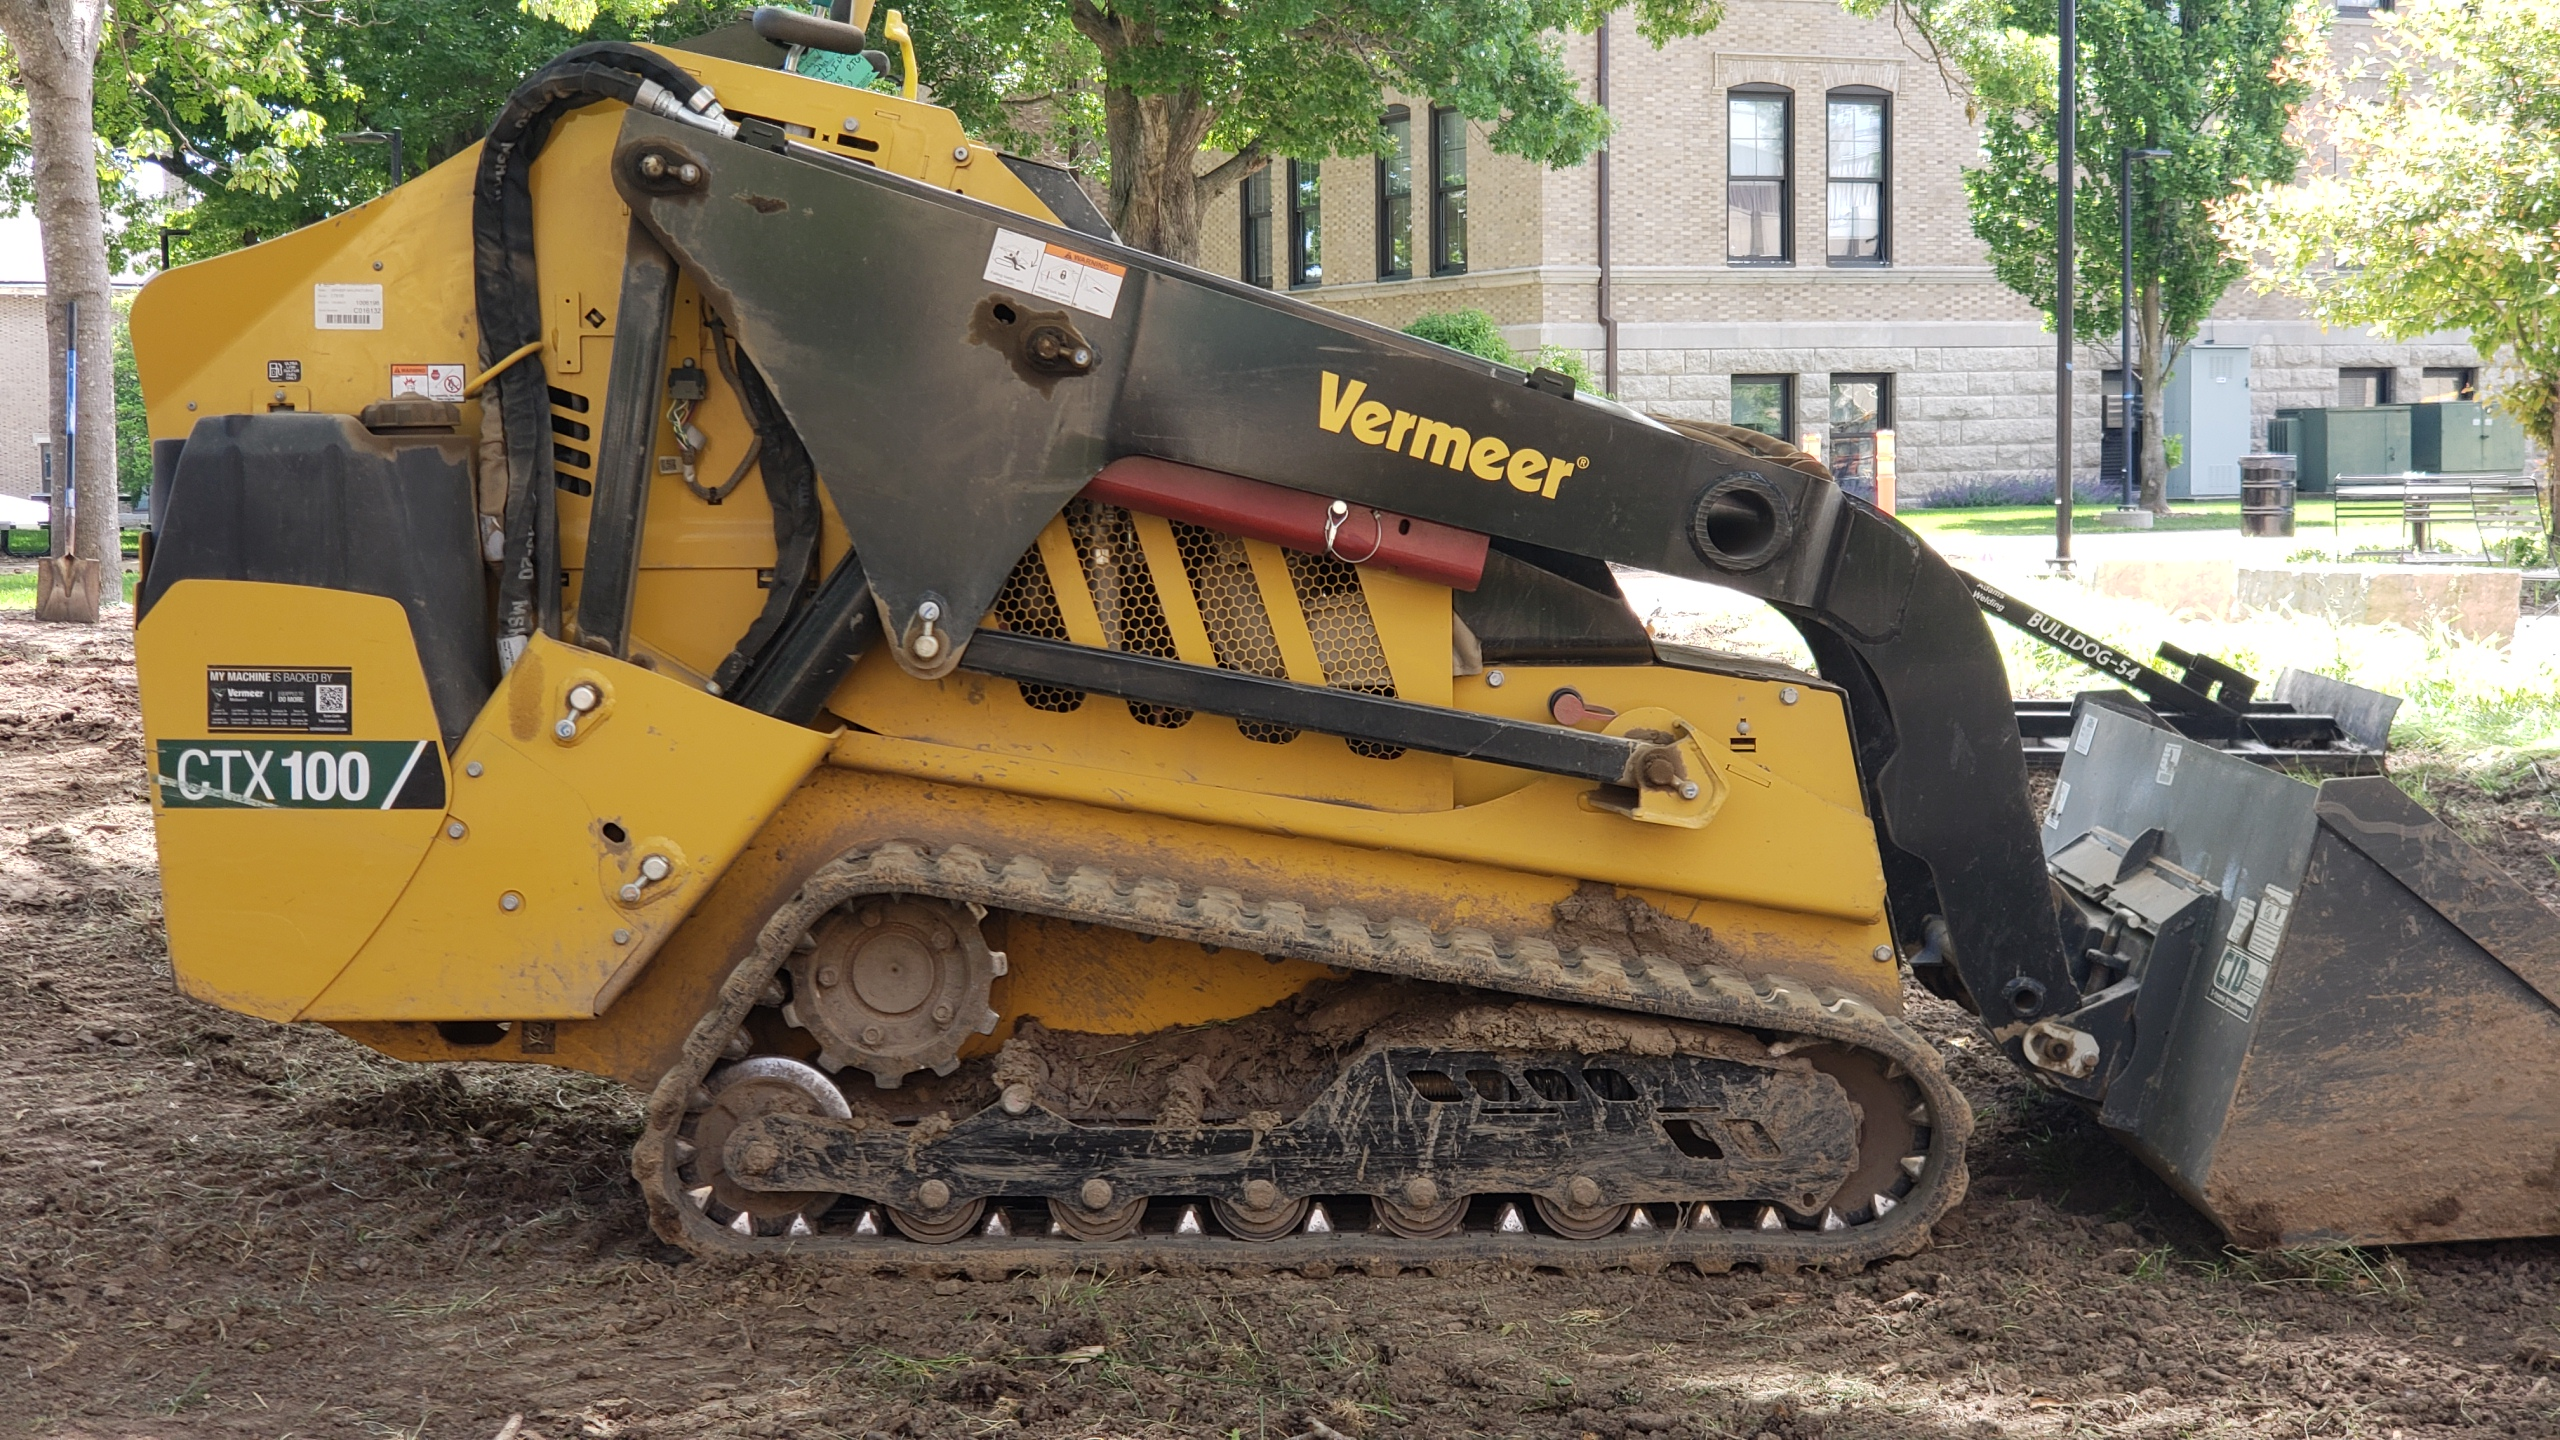
\includegraphics[width=1\linewidth]{SkidSteerBucketLoaderVermeerSide.jpg}
        \caption{Side view of a Skid}\label{fig:sideview}
    \end{figure}
    \FloatBarrier\section*{Mobility}
    Mobility is a measure of how many degrees of freedom a linkage has, and it is calculated with Equation~\eqref{eq:grubler-kutzbach-mobility}, called the Grubler-Kutzbach Mobility equation, where M is the mobility, L is the number of links, J1 is the number of full joints, and J2 is the number of half joints.
    
    \begin{equation}
        \label{eq:grubler-kutzbach-mobility}
        M=3(L-1)-2J_1-J_2
    \end{equation}
    
    A link is a single rigid body. A full joint is a joint with 1 degree of freedom, like a pin or two flat surfaces sliding along each other. A half joint is a joint with 2 degrees of freedom, like a pin in a joint, or two curved surface rolling or slipping along each other. On a kinematic diagram of a linkage, each link is marked with a unique plain number from 1 to the number of links, each full joint is marked with a unique circled number from 1 to the number of full joints, and each half joint is marked with a unique boxed number from 1 to the number of half joints. As shown in \autoref{fig:mobility}, the main linkage of the skid-steer has 6 links, 7 full joints, and 0 half joints. Using the mobility equation as shown in Equation~\eqref{eq:mobility-solution}, the mobility is calculated to be 1.

    \begin{equation}
        \label{eq:mobility-solution}
        M=3(L-1)-2J_1-J_2=3(6-1)-2*7-0=1
    \end{equation}
    
    Because the mobility is 1, only one input is needed to control the linkage. In this case, the input is a hydraulic piston, which is a combination of links 4 and 6\@. \autoref{fig:AnnotatedLinkage} shows the annotated linkage diagram overlain on the original image of the skid-steer.
    
    \FloatBarrier\begin{figure}[ht]
        \centering
        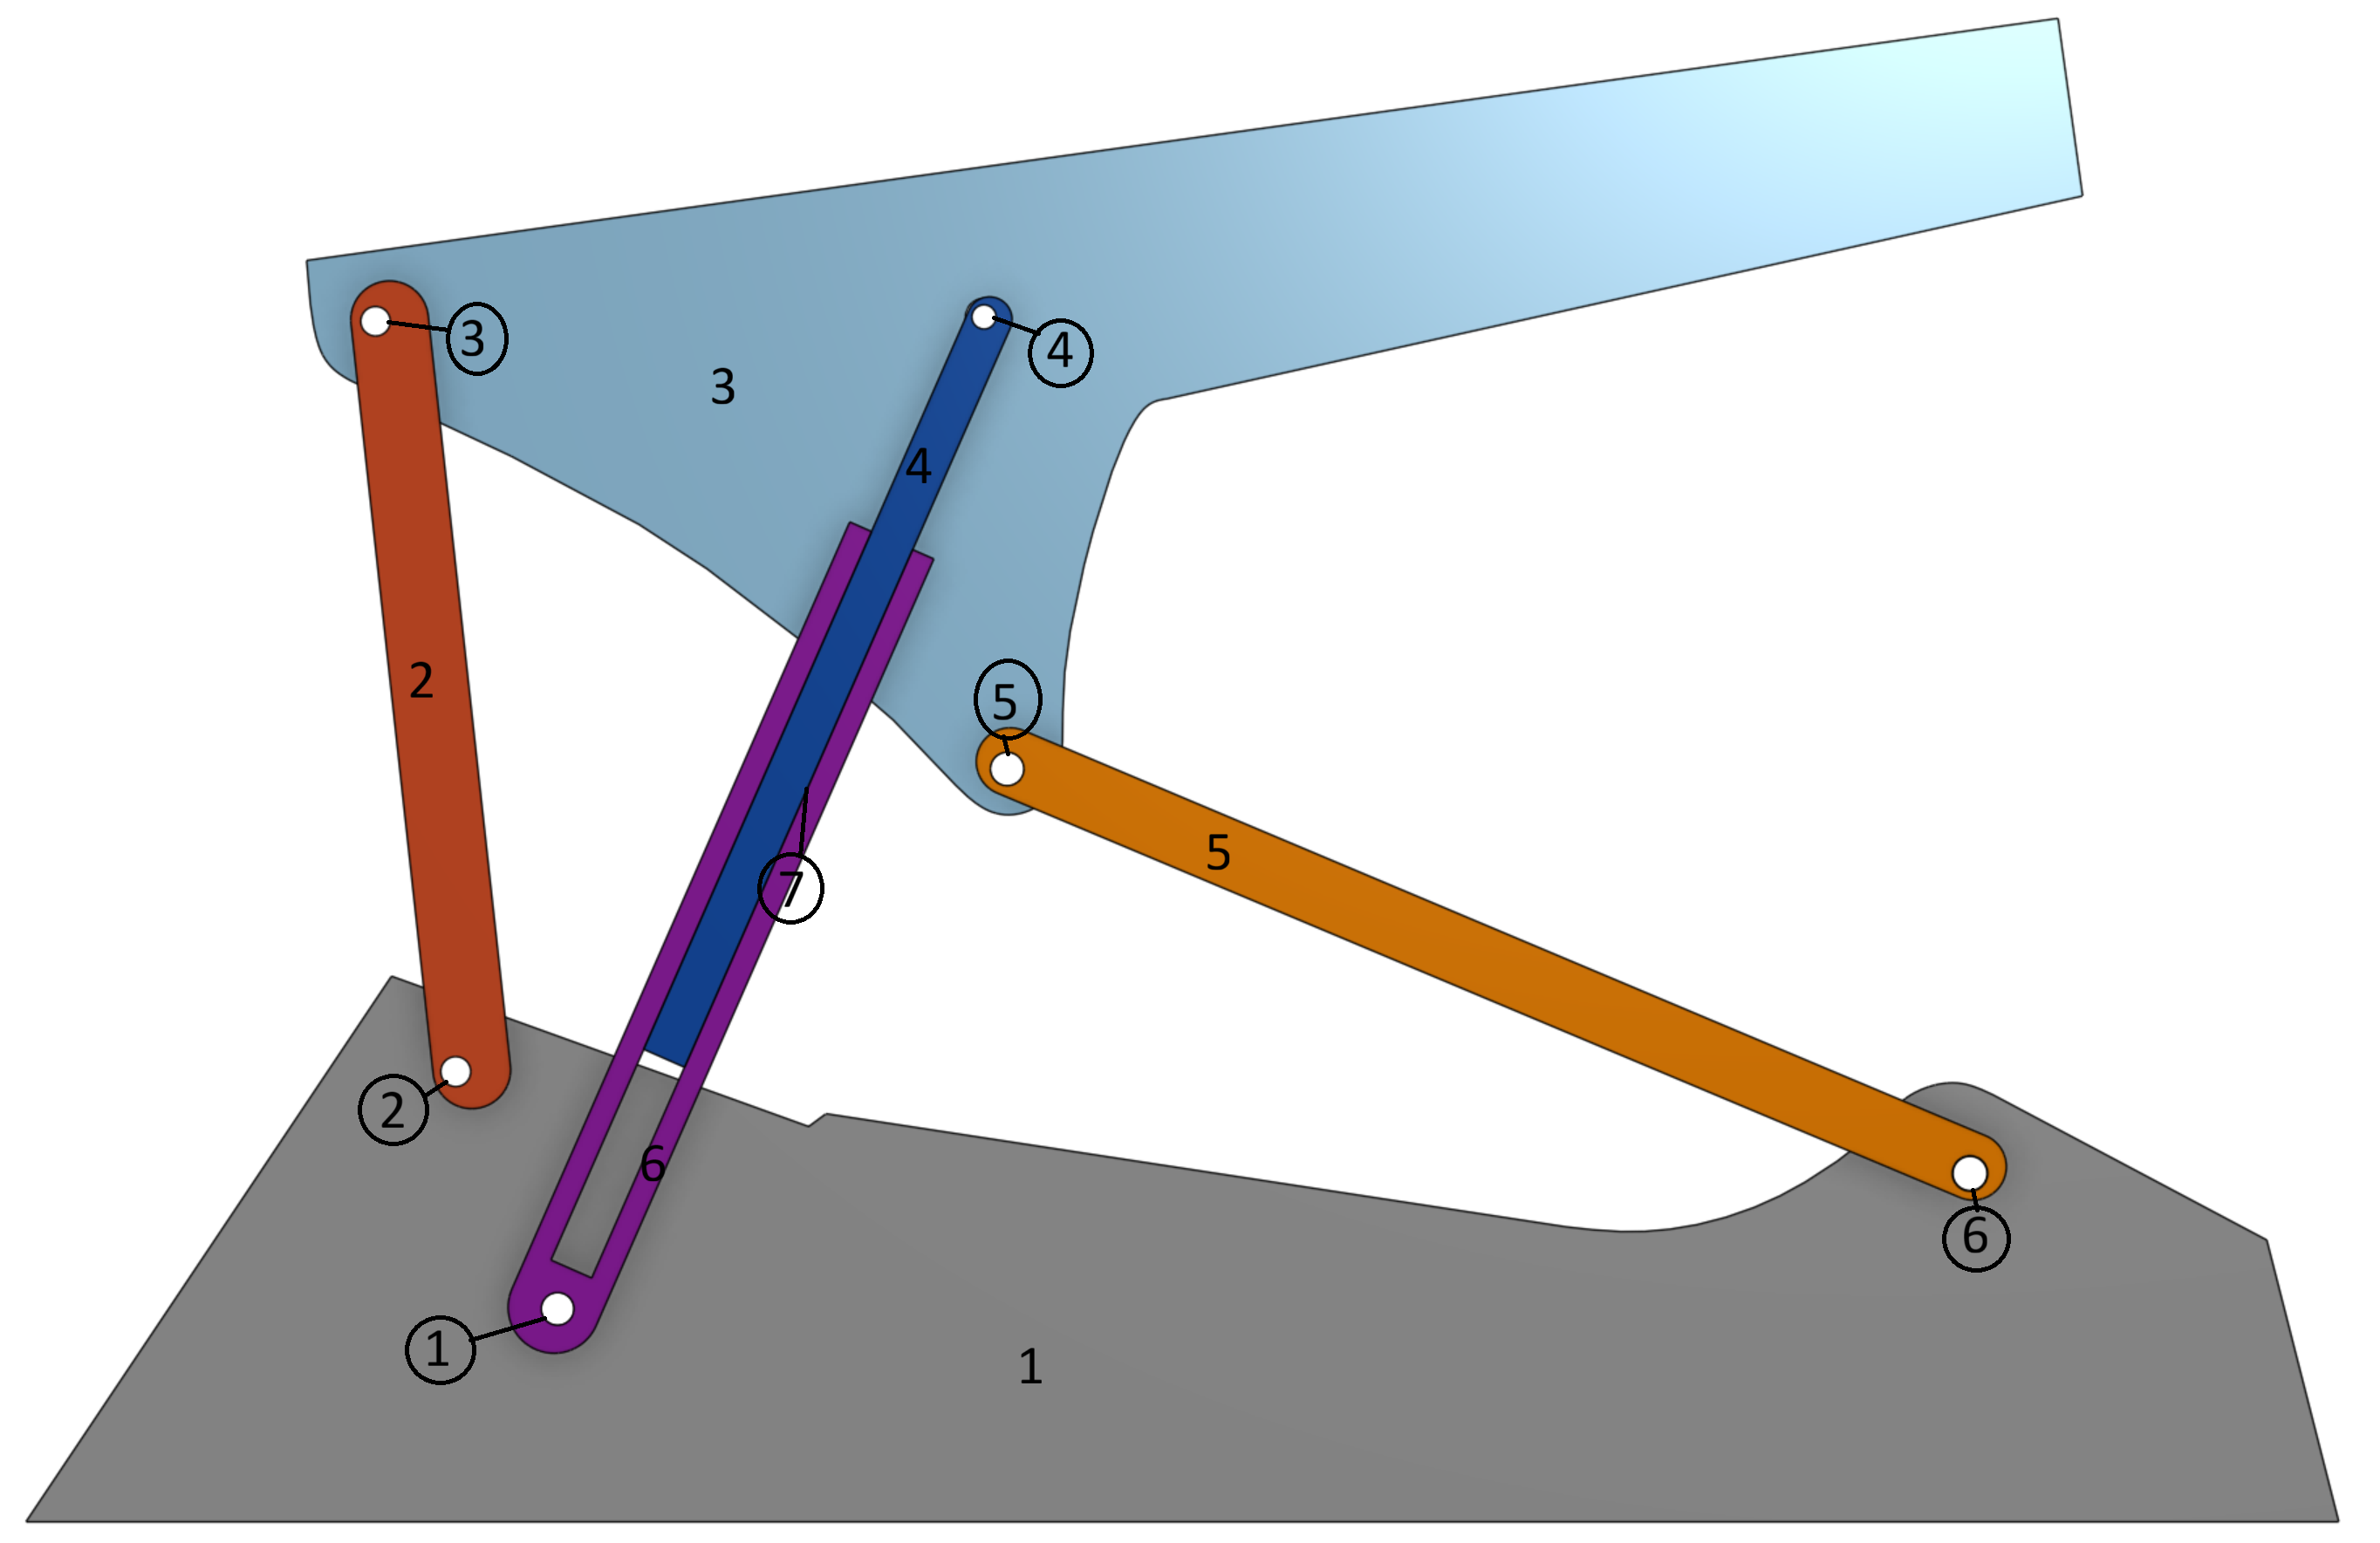
\includegraphics[width=1\linewidth]{HonorsAnnotatedLinkage.png}
        \caption{Annotated Linkage}\label{fig:mobility}
    \end{figure}

    \begin{figure}[t]
        \centering
        \includegraphics[width=1\linewidth]{LinkageAnnotation.png}
        \caption{Annotated Linkage Overlain On Skid-Steer}\label{fig:AnnotatedLinkage}
    \end{figure}

    \FloatBarrier\section*{Multiloop Closure Equations}
    Mobility allows us to determine the degrees of freedom of a linkage, but usually we also need to determine the positions and angles of the individual links. To do this, we can use a method called Multiloop closure. It consists of drawing vectors between joints of each link, then writing equation summing loops of vectors, because the RHS of the equation has to equal zero. This is because the last vector ends where the first vector starts. These vector equations can then be turned into their scalar forms, which can be combined with equations relating rigid geometry of the links, providing a system of equations to solve. When done correctly, the number of unknowns minus the number of scalar and rigid geometry equations should equal the mobility. For the examined linkage, the vectors and loops are labeled as shown in \autoref{fig:multiloop}. The vector equations are shown below as \cref{eq:vector-equation1,eq:vector-equation2}.
    
    \begin{equation}
        \label{eq:vector-equation1}
        \vec{R_{BA}}+\vec{R_{DB}}-\vec{R_{CA}}-\vec{R_{GC}}-\vec{R_{DG}}=0
    \end{equation}

    \begin{equation}
        \label{eq:vector-equation2}
        \vec{R_{GC}}+\vec{R_{DG}}-\vec{R_{DE}}-\vec{R_{EF}}-\vec{R_{FC}}=0
    \end{equation}

    These equations can be expanded into their scalar forms as shown in \cref{eq:scalar-equation1-1,eq:scalar-equation1-2,eq:scalar-equation2-1,eq:scalar-equation2-2,eq:rigid-geometry1,eq:rigid-geometry2} below, where each \(\theta\) is measured counter-clockwise from the horizontal to the tail of the corresponding vector. 
    \begin{equation}
        \label{eq:scalar-equation1-1}
        R_{BA}\cos\theta_{BA}+R_{DB}\cos\theta_{DB}-R_{CA}\cos\theta_{CA}-R_{GC}\cos\theta_{GC}-R_{DG}\cos\theta_{DG}=0
    \end{equation}

    \begin{equation}
        \label{eq:scalar-equation1-2}
        R_{BA}\sin\theta_{BA}+R_{DB}\sin\theta_{DB}-R_{CA}\sin\theta_{CA}-R_{GC}\sin\theta_{GC}-R_{DG}\sin\theta_{DG}=0
    \end{equation}

    \begin{equation}
        \label{eq:scalar-equation2-1}
        R_{GC}\cos\theta_{GC}+R_{DG}\cos\theta_{DG}-R_{DE}\cos\theta_{DE}-R_{EF}\cos\theta_{EF}-R_{FC}\cos\theta_{FC}=0
    \end{equation}

    \begin{equation}
        \label{eq:scalar-equation2-2}
        R_{GC}\sin\theta_{GC}+R_{DG}\sin\theta_{DG}-R_{DE}\sin\theta_{DE}-R_{EF}\sin\theta_{EF}-R_{FC}\sin\theta_{FC}=0
    \end{equation}

    \begin{equation}
        \label{eq:rigid-geometry1}
        \theta_{GC}-\theta_{DG}=0
    \end{equation}

    \begin{equation}
        \label{eq:rigid-geometry2}
        \theta_{DB}+\beta_D-\theta_{DE}=0
    \end{equation}
    
    In these equations, \(R_{BA}\), \(R_{DB}\), \(R_{CA}\), \(\theta_{CA}\), \(R_{GC}\), \(R_{DE}\), \(R_{EF}\), \(R_{FC}\), \(\theta_{FC}\), and \(\beta_D\) are known from the geometry of the linkage and do not change. This leaves \(\theta_{BA}\), \(\theta_{DB}\), \(\theta_{GC}\), \(R_{DG}\), \(\theta_{DG}\), \(\theta_{DE}\), and \(\theta_{EF}\) as unknowns for a total of 7 unknowns. Taking 7 unknowns minus 6 equations yields 1 degree of freedom, which agrees with the earlier mobility analysis. Also, \(R_{DG}\) will be the input because it is controlled by a hydraulic piston.
    
    \begin{figure}[ht]
        \centering
        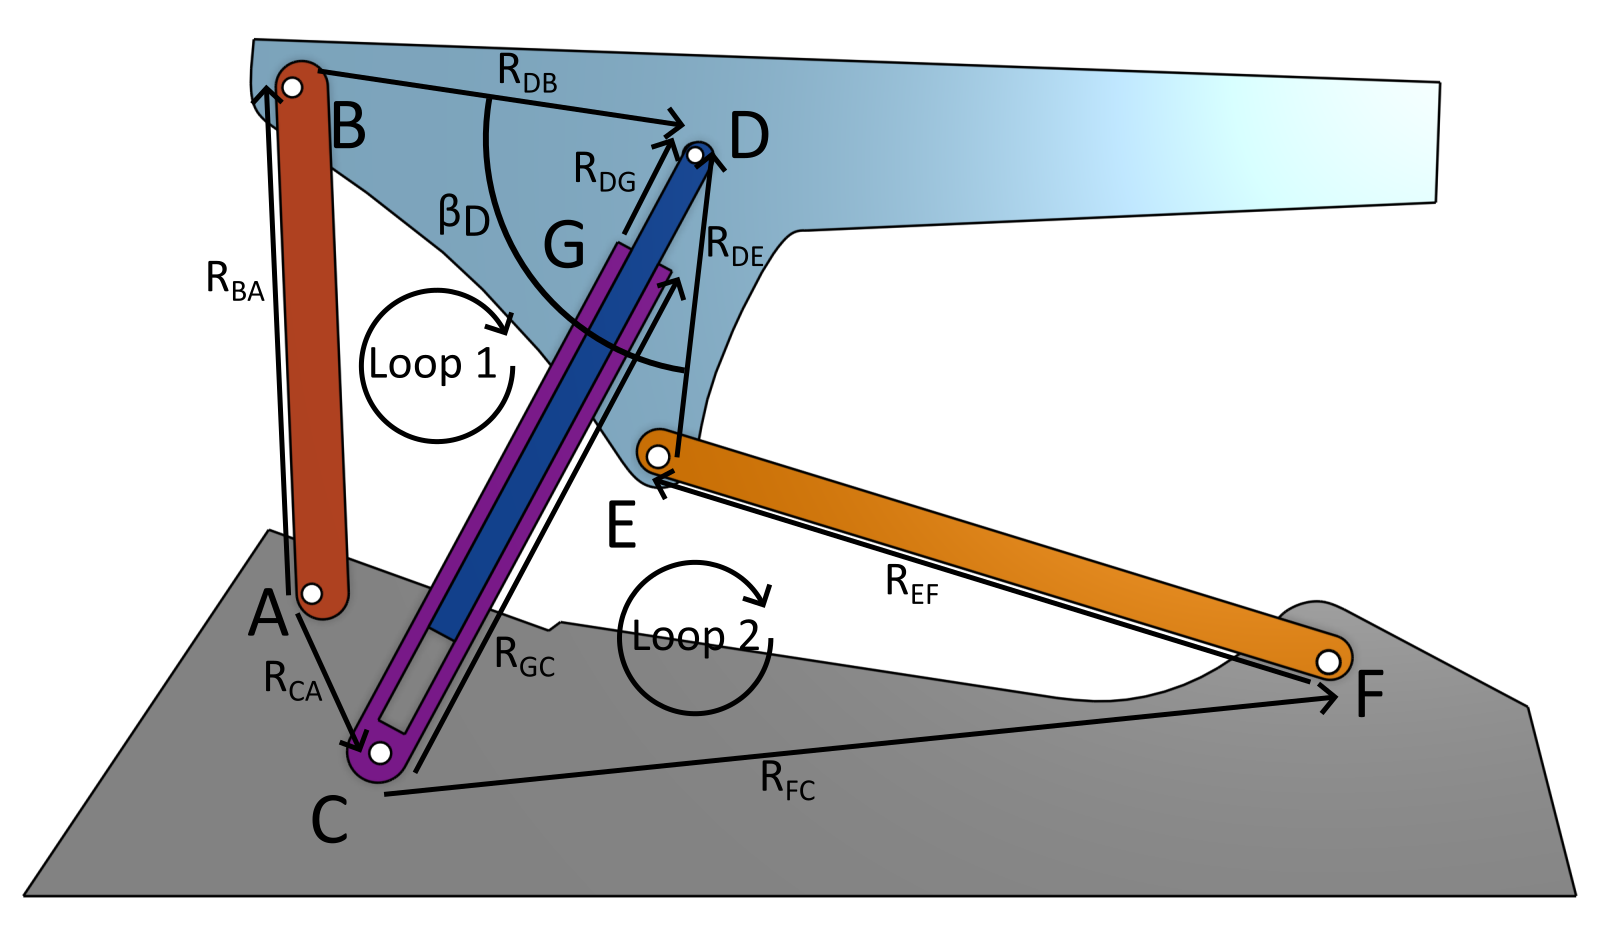
\includegraphics[width=1\linewidth]{MultiLoopClosureAnnotated.png}
        \caption{Diagram showing vector for Multiloop Equations}\label{fig:multiloop}
    \end{figure}
    \FloatBarrier\section*{Code Introduction}
    To solve these equations, I used Python code taking advantage of the fsolve function from the SciPy library. This is a numerical solver function that takes in a set of equations and initial guesses and outputs a solution. Depending on the initial guess, this solution can be incorrect, or a valid solution but not the correct solution for the actual problem constraints. To increase the chancess significantly of a valid solution being generated, I generated a range of initial condition options for each unknown variable and then generated a solution for every combination of initial conditions. Taking these, I kept only ones that had little error when plugged back into the multiloop equations and each variable was within an estimated range of motion. The known link lengths that were plugged into the equations are shown below, and the input length is shown under that. These measurements are only estimates, however, because I found them by finding the length of the loader in its documentation, then measured the length in a side view image of the loader. I took the ratio of these, then measured each link length and and angle in the picture and multiplied each link length by the ratio to get the estimated actual link length. Angles however are not affected by scaling an image up or down though, so I used the measured angles as they were.
    \FloatBarrier\section*{Link Measurements}
    \begin{align*}
        R_{BA}&=24.4 \text{ in.} \\
        R_{DB}&=19.8 \text{ in.} \\
        R_{CA}&=8.5 \text{ in.} \\
        \theta_{CA}&=293.04^\circ \\
        R_{GC}&=25.5 \text{ in.} \\
        R_{DE}&=14.7 \text{ in.} \\
        R_{EF}&=33.9 \text{ in.} \\
        R_{FC}&=45.9 \text{ in.} \\
        \theta_{FC}&=5.44^\circ \\
        \beta_{D}&=92.47^\circ \\
    \end{align*}

    \FloatBarrier\section*{Input Link Length}
    \begin{equation*}
        R_{DC}=29.72 \text{ in.}
    \end{equation*}
        
    \FloatBarrier\section*{Multiloop Solver Code}
    
    \inputminted[python3=true]{python}{../code/main.py}

    \section*{Multiloop Solver Output}
    \begin{minted}[linenos=false]{pwsh-session}
PS C:\...\Honors> python code/main.py
Theta_BA = 82.2 degrees
Theta_DB = 335.1 degrees
Theta_GC = 52.9 degrees
Theta_DG = 52.9 degrees
Theta_DE = 67.6 degrees
Theta_EF = 170.2 degrees
    \end{minted}

\end{document}